
\chapter{Desenvolvimento}

Este capítulo detalha o desenvolvimento do compilador escrito na linguagem Odin, que torna possível a transformação de equações em documentos \LaTeX{} em código GLSL. Cada etapa do processo é encapsulada em um pacote distinto, estruturado em diretórios conforme a \autoref{estrutura-de-pacotes}. O \texttt{lexer} corresponde à tokenização da linguagem, responsável por converter o texto em tokens identificáveis. O \texttt{parser} realiza a análise sintática, construindo a estrutura gramatical do documento. O \texttt{walker} contém funções essenciais para visualização da árvore de sintaxe abstrata (AST) e checagem de tipos feita pelo \texttt{checker}, executando a travessia da árvore de forma ordenada para geração de código feita pelo pacote \texttt{emitter}. A arquitetura completa do compilador pode ser vista na \autoref{fig-estrutura-geral-compilador}.

\begin{figure}[!ht]
  \caption{\label{fig-estrutura-geral-compilador} \small Estrutura de geral da arquitetura do compilador.}
  \begin{center}
    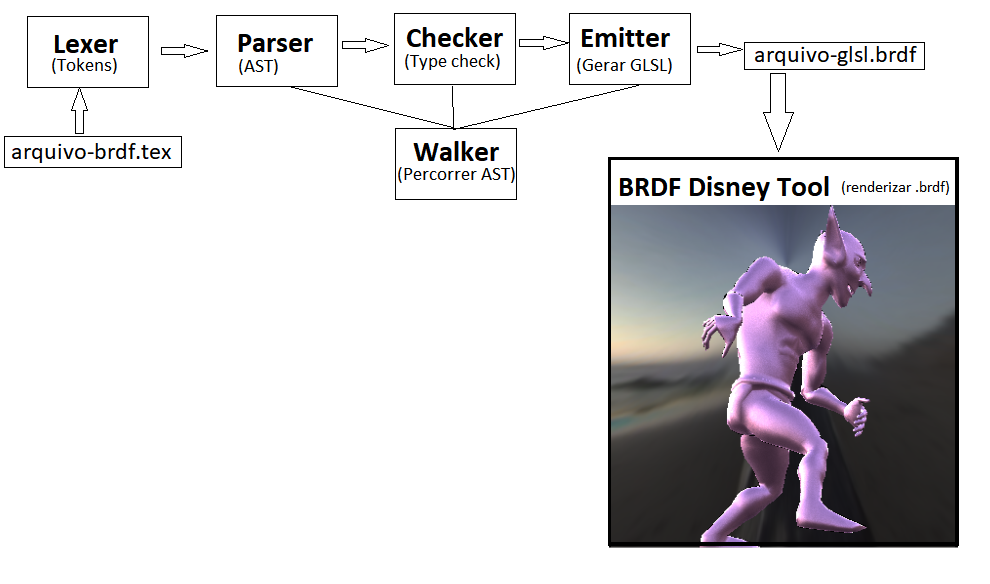
\includegraphics[scale=0.62]{./Imagens/estutura-geral-do-projeto.png}
  \end{center}
\end{figure}


\begin{figure}[!ht]
  \caption{\label{estrutura-de-pacotes} \small Estrutura de pacotes do compilador.}
  \begin{center}
    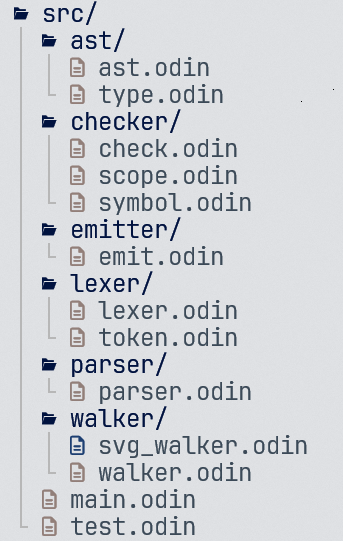
\includegraphics[scale=0.5]{./Imagens/package-structure.png}
  \end{center}
\end{figure}

No módulo \texttt{lexer}, explicado na \autoref{section-lexer}, foi implementado uma análise léxica manual inspirado em máquina de estados para tokenização do documento \LaTeX{}. Este processo converte a entrada textual em uma sequência de tokens, preparando o as estruturas de dados para as próximas etapas de processamento.


Na \autoref{section-parser}, é discutido sobre o pacote \texttt{parser}, que utiliza gramática livre de contexto e a técnica de \textit
{Pratt Parsing} para construir a Árvore de Sintaxe Abstrata (AST). Essa abordagem possibilita uma representação hierárquica precisa das expressões matemáticas de BRDFs, capturando as nuances sintáticas e estruturais do documento original. A especificação da linguagem, apresentada nas \autoref{grammar-ast-pt1} e \autoref{grammar-ast-pt2}, é definida na seção de análise sintática, juntamente com a precedência dos operadores prefixos e infixos.

O componente \texttt{walker}, discutido na \autoref{section-walker}, desempenha funções essenciais para a navegação e análise da Árvore de Sintaxe Abstrata (AST). Suas funcionalidades incluem tanto a visualização da estrutura gerada quanto a preparação para verificações subsequentes por meio do pacote \texttt{checker}. O papel principal do \texttt{walker} é realizar a travessia da AST de forma genérica, oferecendo suporte para decidir se a travessia deve continuar ou se é necessário retornar de um nó antes de alcançar os nós-folha. Além disso, o componente permite a identificação da profundidade atual da travessia e abstrai a forma de percorrer nós de maneira uniforme, independentemente do tipo do nó.

No módulo de \texttt{checker} (\autoref{section-checker}), foi implementado a verificações e inferência de tipos e outras validações semânticas. Este componente garante a consistência e correção das expressões matemáticas antes da geração de código com o auxilio da tabela de simbolos, \autoref{subsection-symbols-scopes}, eliminando potenciais inconsistências ou erros de modelagem. A saída dessa etapa deve está completamente apta a emitir código GLSL e na ordem correta dos Simbolos.

Por fim, o \texttt{emitter} faz uso da AST validada, tabela de símbolos e escopos para gerar código GLSL, transformando expressões matemáticas de BRDFs contidas na AST em um \textit{shader} com toda implementação necessária para ser carregada na ferramenta de visualização Disney Explorer. Os resultados detalhados e experimentos de aplicação do compilador em BRDFs usadas na literatura podem ser consultados no \autoref{chapter.resultados}, onde demonstramos a eficácia da ferramenta na tradução de diversos modelos de BRDFs. Os experimentos também serviram de guia para verificação da corretude da gramática durante seu desenvolvimento.


